\chapter{Metodologi dan Desain Sistem}
  Metode yang akan digunakan pada TA ini adalah Artificial Neural Network. Data hasil analisa Demirbilek et al (2007) \cite{DemirbilekReport} akan dibagi 2. Yakni 80 persen untuk training, dan 20 persen untuk testing. Masing masing, akan disimpan ke dalam file csv. Sistem akan membaca data training langsung dari file, lalu dimasukannya sebagai input ke dalam algoritma ANN. Setelah training, sistem akan menghasilkan suatu model dengan matriks dengan attribut $W_{input}$ dan $W_{output}$ di dalamnya. Tujuannya adalah mendapatkan suatu model yang cukup baik untuk menghasilkan prediksi yang cukup akurat.

\section{Deskripsi Data}
Data yang akan digunakan dalam aplikasi neural network di TA ini adalah data hasil analisis dari eksperimen yang di lakukan oleh US Army Corps of Engineer pada Agustus - September 2006. Analisa dilakukan oleh Demirbilek et al. dan di tulis dalam laporan yang berjudul \emph{"Laboratory Study of Wind Effect on Runup over Fringing Reefs"}.

\subsection{Kondisi Eksperimen}
\label{kondisiEksperimen}

Eksperimen dibagi menjadi 3 bagian. Eksperimen pertama dilakukan hanya menggunakan variabel gelombang, dengan kecepatan angin 0. Eksperimen kedua, dilakukan hanya menggunakan variabel angin. Selanjutnya eksperimen ketiga adalah gabungan dari perubahan variable gelombang dan variabel angin.

\begin{figure}
  \begin{center}
    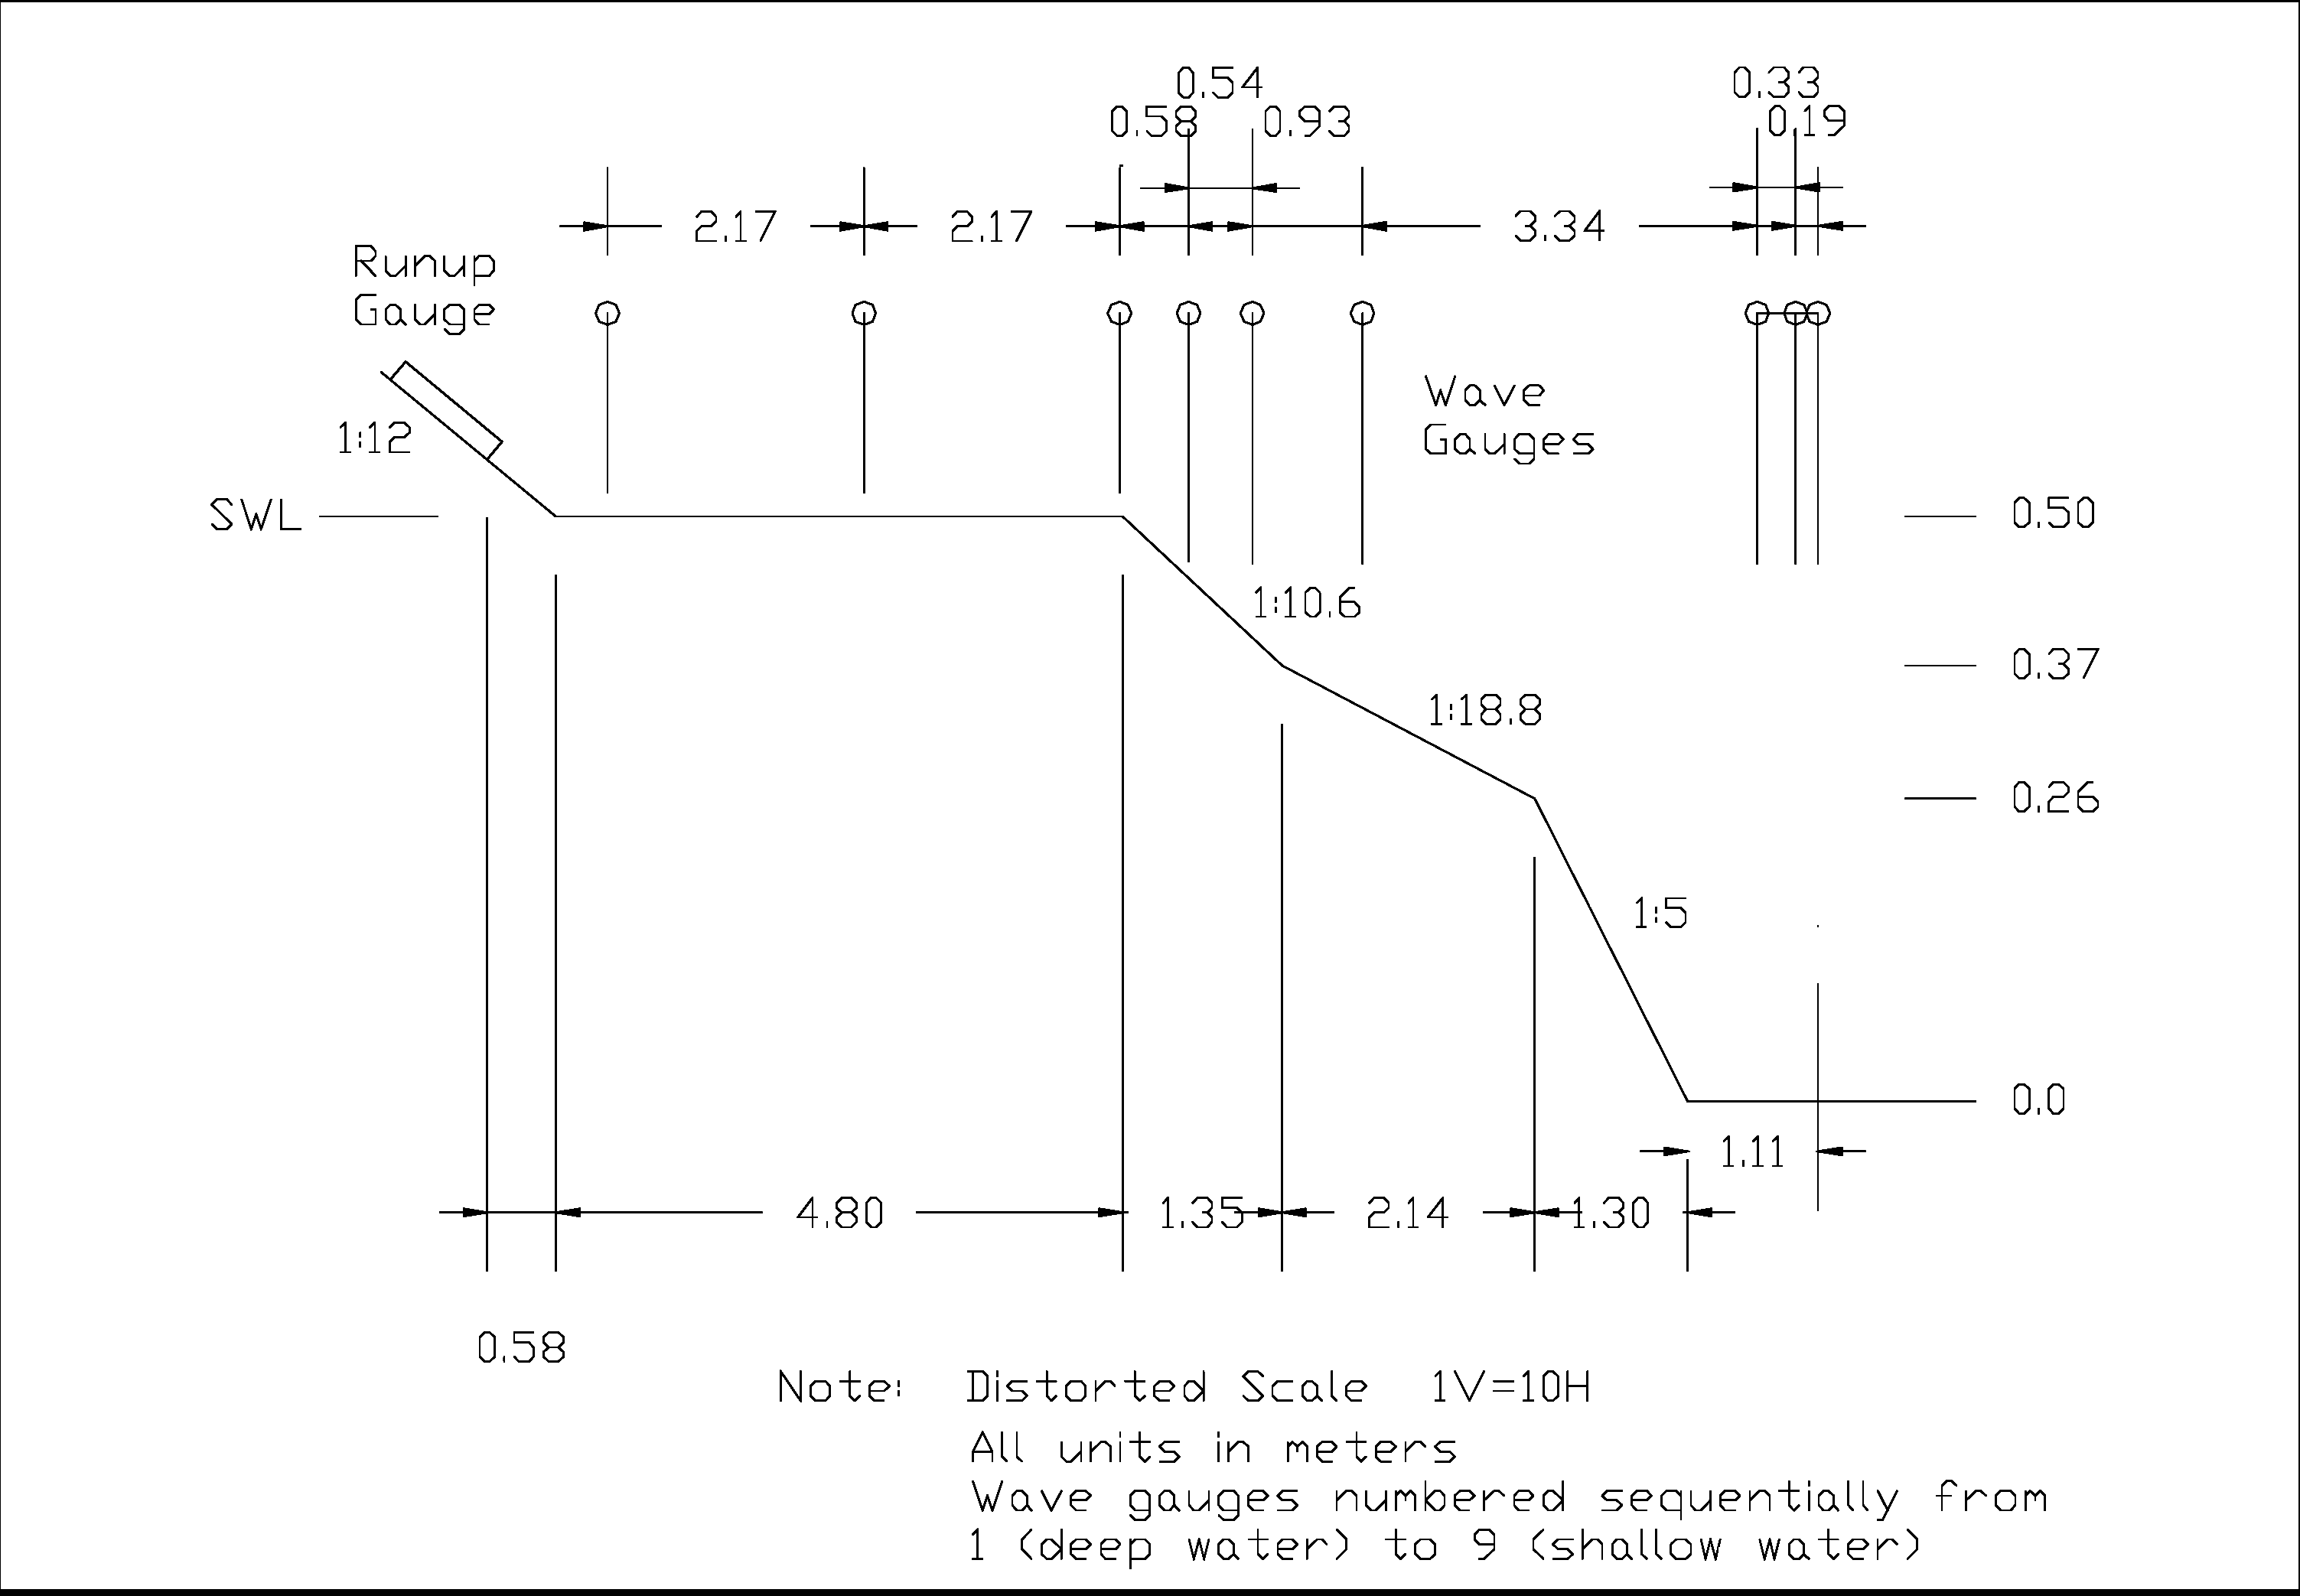
\includegraphics[scale=0.2]{./images/instrumen_eksperimen.png}
  \end{center}
  \caption{}
\end{figure}
\FloatBarrier

Pada eksperimen ini ada 9 sensor gelombang, 2 sensor kecepatan angin, dan 1 sensor \emph{runup} gelombang. Wilayah penyebaran sensor gelombang dikelompokan menjadi 2. Wilayah pertama berada di atas karang dan wilayah kedua berada di laut.. Wilayah karang merupakan gabungan dari wilayah karang yang datar \emph{Reef Flat} dan wilayah karang yang miring. Wilayah karang datar memiliki panjang mulai dari \emph{SWL} hingga 4.8 meter ke arah laut. Wilayah karang yang miring \emph{Reef Slope} di mulai dari bibir karang datar hingga 4.79 meter ke arah laut. Laut didefinisikan dengan wilayah dengan dasar terdalam. Untuk sensor 1, 2, dan 3 tersebar di wilayah laut, sensor 4, 5, dan 6 tersebar di wilayah \emph{reef slope}, dan untuk sensor 7, 8, dan 9 tersebar di wilayah \emph{reef flat}.

\pagebreak

\subsection{Hasil Analisa Data}

Dari laporan \emph{"Laboratory Study of Wind Effect on Runup over Fringing Reefs"} \cite{DemirbilekReport} data yang di hasilkan berupa data hasil analisa yang berasal dari raw data yang merupakan time series. Pada table tersebut $H$ merupakan tinggi gelombang, $T$ merupakan spectral peak periods, $WL$ merupakan Wave Length, dan $R_{max}$ adalah ketinggian maksimum dari \emph{runup}. $H$, $WL$, dan $R_{max}$ merupakan dalam $cm$.

\begin{table}
    \begin{center}
      \begin{tabular}{|l|l|l|l|l|l|l|l|}
      \hline
      TestId & H & T & WL & $R_{max}$ & Wind \\ \hline
      Test99 & 5.5 & 1.25 & 50.0 & 1.5 & 7.1 \\ \hline
      Test100 & 6.0 & 1.0 & 50.0 & 1.6 & 6.9 \\ \hline
      Test101 & 3.3 & 1.0 & 50.0 & 0.7 & 5.3 \\ \hline
      Test102 & 8.2 & 2.5 & 53.1 & 8.4 & 7.0 \\ \hline
      Test103 & 8.6 & 2.0 & 53.1 & 7.8 & 7.1 \\ \hline
      Test104 & 8.0 & 1.75 & 53.1 & 6.7 & 5.8 \\ \hline
      Test105 & 7.8 & 1.5 & 53.1 & 5.9 & 6.3 \\ \hline
      Test106 & 5.4 & 1.5 & 53.1 & 4.0 & 6.7 \\ \hline
      Test107 & 6.3 & 1.25 & 53.1 & 4.5 & 6.8 \\ \hline
      Test108 & 6.6 & 1.0 & 53.1 & 6.4 & 6.7 \\ \hline
      Test109 & 3.8 & 1.0 & 53.1 & 5.3 & 6.5 \\ \hline
      \end{tabular}
    \end{center}
    \caption{Sampel data hasil analisa.}
  \end{table}
\FloatBarrier

\section{Model Artificial Neural Network}
  Pada TA ini, digunakan model ANN dengan 1 hidden layer (\emph{Non-deep Neural Network}). Terdapat 4 input, yang berupa vector dengan masing-masing nilai berupa $H$ (\emph{Significant Height} Gelombang) dalam $cm$, $T$ (\emph{Spectral Peak Periods}) dalam $detik$, $WL$ (\emph{Wave Length}) dalam $cm$, dan $WIND$ (kecepatan angin) dalam $meter/detik$. Model AAN ini memiliki 1 output dan merupakan model \emph{regressi linear}. Output merupakan prediksi ketinggian \emph{runup} dengan satuan $cm$.

  \def\layersep{4cm}
  \begin{figure}
    \begin{tikzpicture}[shorten >=1pt,->,draw=black!50, node distance=\layersep]
        \tikzstyle{every pin edge}=[<-,shorten <=1pt]
        \tikzstyle{neuron}=[circle, fill=black!25,minimum size=17pt,inner sep=0pt]
        \tikzstyle{input neuron}=[neuron, fill=green!50];
        \tikzstyle{output neuron}=[neuron, fill=red!50];
        \tikzstyle{hidden neuron}=[neuron, fill=blue!50];
        \tikzstyle{annot} = [text width=4em, text centered]

        % Draw the input layer nodes
        \node[input neuron, pin=left:H] (I-H) at (0,-1) {};
        \node[input neuron, pin=left:WL] (I-T) at (0,-2) {};
        \node[input neuron, pin=left:WIND] (I-WL) at (0,-3) {};
        \node[input neuron, pin=left:T] (I-WIND) at (0,-4) {};

        % Draw the hidden layer nodes
        \path[yshift=0.0cm]{}
            node[hidden neuron] (H-1) at (\layersep,-1 cm) {};
        \path[yshift=0.0cm]{}
            node[hidden neuron] (H-2) at (\layersep,-2 cm) {};
        \path[yshift=0.0cm]{}
            node[hidden neuron] (H-3) at (\layersep,-3 cm) {};
        \path[yshift=0.0cm]{}
            node[hidden neuron] (H-4) at (\layersep,-4 cm) {};

        % Draw the output layer node
        \node[output neuron,pin={[pin edge={->}]right:Prediksi Runup}, right of=H-3] (O) {};

        % Connect every node in the input layer with every node in the
        % hidden layer.
        \foreach \source in {H, T, WL, WIND}
            \foreach \dest in {1,...,4}
                \path (I-\source) edge node[midway, right] {$W_{hidden}$} (H-\dest);

        % Connect every node in the hidden layer with the output layer
        \foreach \source in {1,...,4}
            \path (H-\source) edge node[midway, right] {$W_{output}$} (O);

        % Annotate the layers
        \node[annot,above of=H-1, node distance=1cm] (hl) {Hidden layer};
        \node[annot,left of=hl] {Input layer};
        \node[annot,right of=hl] {Output layer};
        \label{modelANNTA}
    \end{tikzpicture}
    \caption{Model ANN yang digunakan pada TA ini.}
  \end{figure}
  \FloatBarrier

\section{Flowchart Sistem TA}

Secara keseluruhan, terdapat bentuk hirarki dalam sistem ini. Hirarki \emph{root} (Hirarki Utama), yakni sistem itu sendiri, bertugas sebagai pengatur. \emph{Root} memiliki anak yang memiliki tugas-tugas tertentu, seperti: \emph{Membaca File}, \emph{Transformasi Data}, \emph{Membagi Data}, atau yang paling penting yakni \emph{Training Data}.

\subsection{Flowchart Sistem Utama}

  Sistem utama merupakan pengatur dari komponen-komponen yang ada pada sistem TA ini. Komponen-komponen tersebut termasuk: Pembacaan Data, Transformasi Data, Pembagian Data, Inisialisasi Epoch Dan Learning Rate, Melakukan Training, dan Melakukan Testing.

  Sistem dimulai dengan membaca data. Pembacaan data dibagi menjadi 2. Pembacaan data training dan pembacaan data testing. Data training mencakup 80 persen dari seluruh data observasi, sedangkan data training mencakup 20 persen. Hal ini sejalan dengan Fan et al \cite{fan2008liblinear}, dimana beliau menggunakan rasio 80/20 untuk training dan testing. Setelah melakukan pembacaan data, sistem akan melakukan transformasi data. Mengubah data csv, menjadi matriks dengan panjang kolom 4, yang mewakili $H$, $T$, $WL$, dan $WIND$. Komponen selanjutnya adalah inisialisasi \emph{epoch} dan \emph{learning rate}. \emph{Epoch} adalah representasi dari keseluruhan data yang digunakan pada training. Sedangkan \emph{learning rate} adalah besaran dari suatu langkah pembelajaran. Nilai dari \emph{learning rate} dan \emph{epoch} selanjutnya akan dimasukan ke dalam fungsi training. 

\begin{figure}[ht]
  \caption{Flowchart Sistem Utama}
  \begin{center}
    \tikzstyle{decision} = [diamond, draw, 
        text width=4.5em, text badly centered, node distance=3cm, inner sep=0pt]
    \tikzstyle{block} = [rectangle, draw, 
        text width=12em, text centered, minimum height=2em]
    \tikzstyle{circle} = [draw, ellipse, minimum height=2em, distance=4em]
    \tikzstyle{blockTraining} = [rectangle, draw, fill=red!20, 
        text width=12em, text centered, minimum height=2em]
    \tikzstyle{line} = [draw, -latex']
        
    \begin{tikzpicture}[node distance = 2.3cm, auto]
        % Place nodes
        \node [circle] (init) {Mulai};
        \node [block, below of=init] (bacaData) {Membaca data report dari csv file};
        \node [block, below of=bacaData] (transformasiData) {Transformasi data menjadi matrix};
        \node [block, below of=transformasiData] (setupEpochLr) {Menentukan jumlah epoch dan learning rate};
        \node [blockTraining, below of=setupEpochLr] (training) {Melakukan Training};
        \node [blockTraining, below of=training] (testing) {Melakukan Testing};
        \node [circle, below of=testing] (stop) {Stop};
      
        % Draw edges
        \path [line] (init) -- (bacaData);
        \path [line] (bacaData) -- (transformasiData);
        \path [line] (transformasiData) -- (setupEpochLr);
        \path [line] (setupEpochLr) -- (training);
        \path [line] (training) -- (testing);
        \path [line] (testing) -- (stop);
        \label{fig:sistem}
    \end{tikzpicture}
  \end{center}
\end{figure}
\FloatBarrier

\subsection{Flowchart Komponen Training Dan Testing}
\label{FlowChartTraining}
Pada bagian training dan testing \ref{fig:sistem}, algoritma yang digunakan adalah algoritma ANN. Untuk testing, hanya dilakukan algoritma \emph{Feed Forward}.

Algoritma ANN dimulai dengan inisialisasi weight dengan random data. Selanjutnya, nilai pada \emph{input parameter} akan dikalikan dengan $weight$ \emph{hidden layer} $W^1$, sehingga dihasilkan $a^1$. Untuk menjadi nilai pada \emph{neuron hidden layer} $z^1$, $a$ akan diaktifasi dengan fungsi aktivasi $RELU$ sehingga nilai $z^1$ merupakan hasil dari $relu(a)$. Untuk mengahasilkan nilai prediksi, $z^1$ dikalikan dengan $weight$ pada \emph{output} $W^2$, sehingga mengasilkan $a^2$. Nilai $a^2$ merupakan nilai hasil prediksi, karna fungsi aktivasi dari \emph{output} adalah linear ($f(a) = a$).

\begin{figure}[ht]
  \caption{Flowchart Komponen Training Dan Testing}
  \begin{center}
    \tikzstyle{block} = [rectangle, draw, fill=blue!20, 
        text width=10em, text centered, minimum height=6em]
    \tikzstyle{blockTraining} = [rectangle, draw, fill=red!20, 
        text width=14em, text centered, minimum height=2em]
    \tikzstyle{stopTrainng} = [rectangle, draw, fill=red!20, 
        text width=3em, text centered,  distance=10cm]
    \tikzstyle{line} = [draw, -latex']
    \tikzstyle{circle} = [draw, ellipse, minimum height=2em, distance=4em]
    \tikzstyle{decision} = [diamond, draw, fill=blue!20, 
        text width=4em, text badly centered, node distance=2.5cm, inner sep=0pt]
        
    \begin{tikzpicture}[node distance = 2cm, auto]
        % Place nodes
        \node [circle] (init) {Mulai};
        \node [blockTraining, below of=init] (randomWeight) {Inisialisasi $weight$ dengan random data};
        \node [blockTraining, below of=randomWeight] (IW){Mengalikan Input Layer Dengan $Weight$ hidden layer};
        \node [blockTraining, below of=IW] (aktivasi){Jalankan fungsi aktivasi hidden layer};
        \node [blockTraining, below of=aktivasi] (HW){Mengalikan Input Layer Dengan $Weight$ untuk $output$};
        \node [blockTraining, below of=HW] (aktivasiOutput){Menjalankan fungsi aktivasi untuk output neuron};
        \node [blockTraining, below of=aktivasiOutput] (cost){Kalkulasi Error};
        \node [circle, below of=cost] (stop){Stop};
  
        % Draw edges
        \path [line] (init) -- (randomWeight);
        \path [line] (randomWeight) -- (IW);
        \path [line] (IW) -- (aktivasi);
        \path [line] (aktivasi) -- (HW);
        \path [line] (HW) -- (aktivasiOutput);
        \path [line] (aktivasiOutput) -- (cost);
        \path [line] (cost) -- (stop);
    \end{tikzpicture}
  \end{center}
\end{figure}
\FloatBarrier
